\section{标准库}
我们用整本书来宣传编写我们自己的代码的艺术。 现在我们终于承认一些伟大的程序员已经编写了我们可以使用的代码。 
库是完成我们工作的最佳方式。 这并不是因为懒惰,而是因为有更好的事情要做,而不是重新发明别人的工作。

本章涵盖三组不同的库函数:

\begin{enumerate}
	\item SYCL规范定义的内置函数

	\item C++标准库

	\item C++17并行算法,由oneAPI DPC++库(oneDPL)支持
\end{enumerate}

SYCL 定义了一组丰富的内置函数,提供主机和设备代码共享的通用函数。 
所有 SYCL 实现都支持这些函数,因此我们可以依赖所有 SYCL 设备上可用的关键数学库。

不保证所有 SYCL 实现在设备代码中都支持 C++ 标准库。 
然而,DPC++ 编译器(和其他编译器)支持将此作为 SYCL 的扩展,因此我们在这里简要讨论该扩展的局限性。

最后,oneAPI DPC++ 库 (oneDPL) 提供了一组基于 C++17 算法的算法,并在 SYCL 中实现,
为 SYCL 程序员提供高生产力的解决方案。 这可以最大限度地减少跨 CPU、GPU 和 FPGA 的编程工作。 
尽管 oneDPL 不是 SYCL 2020 的一部分,但由于它是在 SYCL 之上实现的,因此它应该与任何 SYCL 2020 编译器兼容。

\subsection{内置函数}
SYCL 提供了一组丰富的内置函数,支持各种数据类型。 这些内置函数在主机和设备上的 sycl 命名空间中可用,可分为以下几类:

\begin{itemize}
	\item 浮点数学函数:asin、acos、log、sqrt、floor 等。

	\item 整数函数:abs、max、min 等。

	\item 常用函数:clamp、smoothstep等。

	\item 几何函数:cross, dot, distance等。

	\item 关系函数:isequal、isless、isfinite 等。
\end{itemize}

有关此广泛函数集合的文档可以在 SYCL 2020 规范中找到,
在线文档位于registry.khronos.org/SYCL/specs/sycl-2020/html/sycl-2020.html 的第 4.17.5 至 4.17.9 节中。

一些编译器可能提供选项来控制这些函数的精度。 
例如,DPC++ 编译器提供了多个此类选项,包括 -mfma、-ffast-math 和 -ffp-contract=fast。 
检查 SYCL 实现的文档以了解类似选项(及其默认值)的可用性非常重要。

一些 SYCL 内置函数在 C++ 标准库中具有等效函数(例如 sycl::log 和 std::log)。 
SYCL 实现不需要支持在设备代码中调用 C++ 标准库函数,但某些实现(例如 DPC++)可以。

\begin{figure}[H]
	\centering
	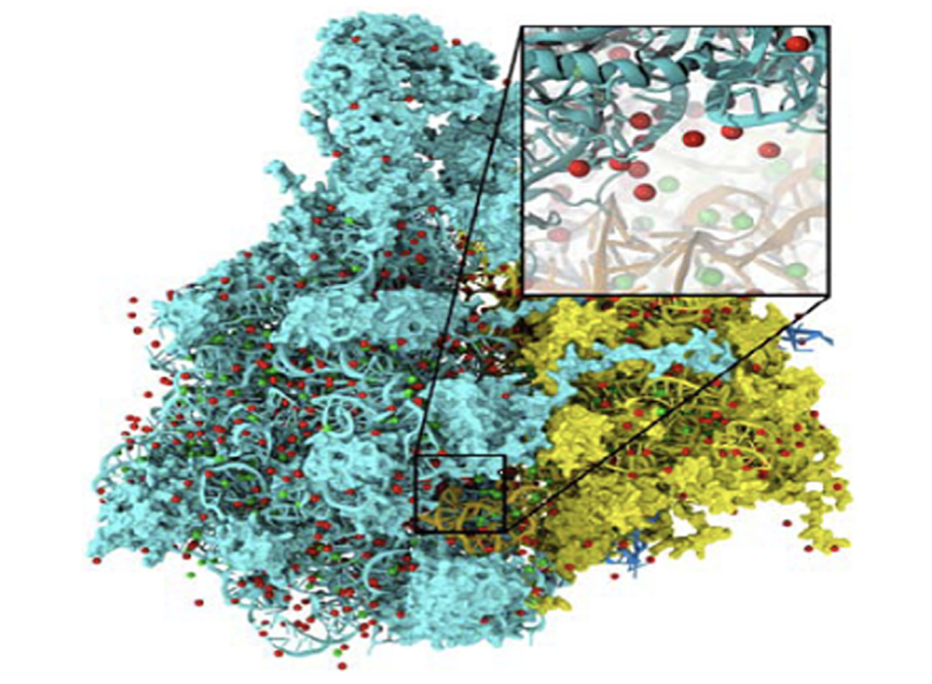
\includegraphics[width=0.9\textwidth]{figs/F18.1.png}
	\caption{\textit{使用 std::log 和 sycl::log }}
\end{figure}

图 18-1 演示了 C++ std::log 函数和 SYCL 内置 sycl::log 函数在设备代码中的用法。 
使用 DPC++ 编译器实现,两个函数产生相同的数值结果。 
在示例中,内置关系函数 sycl::isequal 用于比较 std::log 和 sycl::log 的结果。

请注意,SYCL 2020 规范并不要求 SYCL 数学函数实现必须针对给定硬件目标
生成与其对应的 C 和 C++ 标准数学函数完全相同的数值结果。 
该规范允许在实现中进行某些变化,以考虑不同硬件平台的特性和限制。 
因此,SYCL 实现在实践中可能会产生匹配结果,如图 18-1 中的代码示例所示。

\subsubsection{使用带有内置函数的 sycl:: 前缀}
我们强烈建议调用 SYCL 内置函数,并在名称前添加显式 sycl:: 。 
仅调用 sqrt() 并不能保证调用所有实现上内置的 SYCL,即使“using namespace sycl;” 已经用过。

\begin{remark}
	SYCL 内置函数应始终在内置名称前面使用显式 sycl:: 进行调用。不遵循此建议可能会导致奇怪且不可移植的结果。
\end{remark}

在编写可移植代码时,我们建议避免使用命名空间 sycl; 完全赞成显式使用 std:: 和 sycl:: 命名空间。 
通过明确,我们消除了在某些 SYCL 实现中遇到无法解决的冲突的可能性。 
这也可能使代码将来更容易调试(例如,如果实现为 std:: 和 sycl:: 命名空间中的数学函数提供不同的精度保证)。

\subsection{C++ 标准库}
如前所述,SYCL 规范不保证设备代码支持 C++ 标准库中的函数。 
然而,有几个编译器确实支持这些函数:这简化了现有 C++ 代码到 SYCL 设备的卸载,
并使编写使用 SYCL 作为实现细节的库变得更容易(
例如,将函数传递到库中的用户可以编写 该函数无需使用任何 SYCL 特定函数)。

\begin{remark}
	由于设备代码中对 std:: 命名空间函数的支持因 SYCL 实现而异,
	因此我们无法确定采用 C++ 标准库的内核是否可以跨多个 SYCL 编译器和实现移植。
\end{remark}

DPC++ 编译器与一组经过测试的 C++ 标准 API 兼容——我们只需包含相应的 C++ 头文件并使用 std 命名空间即可。 
所有这些 API 都可以在设备Kernel中使用,就像在典型的 C++ 主机应用程序中使用一样。 
图 18-2 显示了如何在设备代码中使用 std::swap 的示例。

\begin{figure}[H]
	\centering
	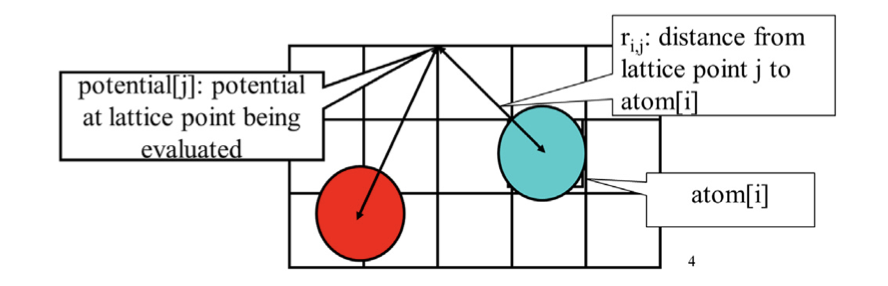
\includegraphics[width=0.9\textwidth]{figs/F18.2.png}
	\caption{\textit{在设备代码中使用 std::swap }}
\end{figure}

图 18-3 列出了带有“Y”的 C++ 标准 API,表示在撰写本文时,
这些 API 已在 CPU、GPU 和 FPGA 设备的 SYCL Kernel中进行了测试。 
空白表示本书出版时覆盖不完整(并非所有三种设备类型)。

\begin{figure}[H]
	\centering
	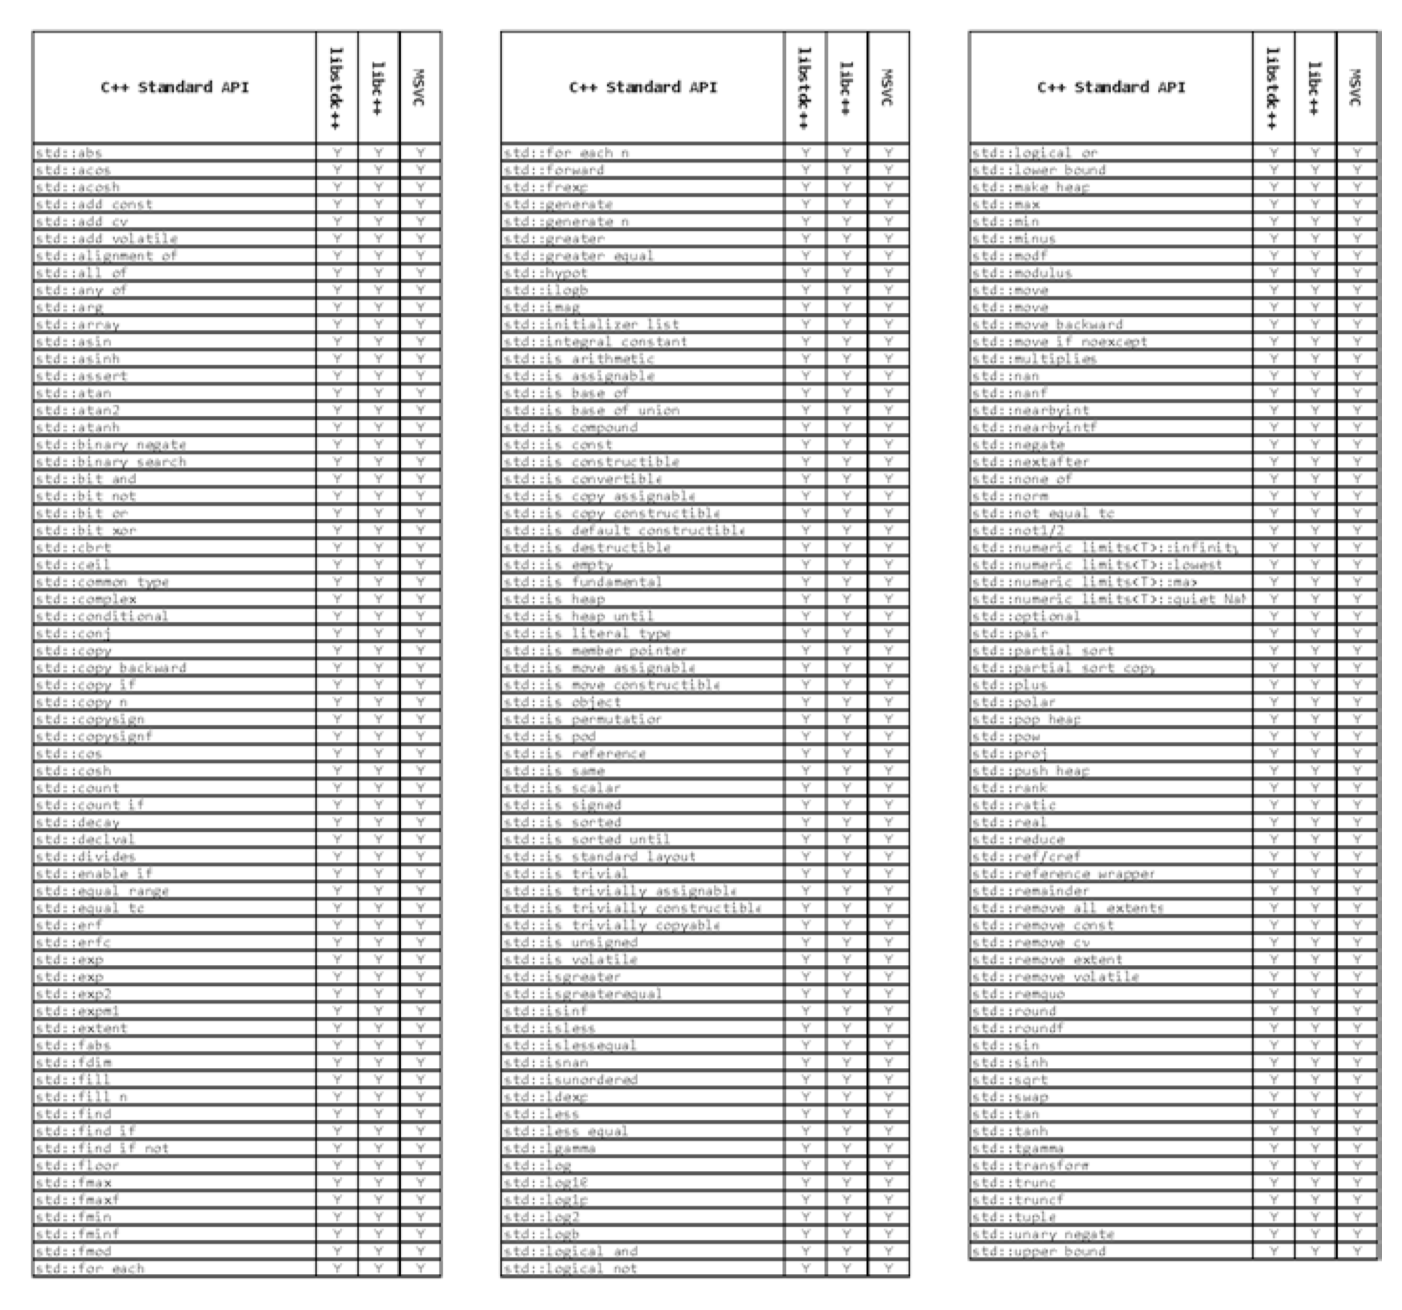
\includegraphics[width=0.9\textwidth]{figs/F18.3.png}
	\caption{\textit{支持 CPU/GPU/FPGA 的库(在图书出版时) }}
\end{figure}

经测试的标准 C++ API 在带有 gcc 7.5.0+ 的 libstdc++ (GNU) 
和带有 clang 11.0+ 的 libc++ (LLVM) 
以及带有用于主机 CPU 的 Microsoft Visual Studio 2019+ 的 MSVC 标准 C++ 库中受支持。

在 Linux 上,GNU libstdc++ 是 DPC++ 编译器的默认 C++ 标准库,因此不需要编译或链接选项。

如果我们想使用 libc++,请使用编译选项 -stdlib=libc++ -nostdinc++ 来利用 libc++ 
并且不包含系统中的 C++ std 标头。 
DPC++ 编译器已在 Linux 上的 SYCL Kernel中使用 libc++ 进行了验证,
但运行时需要使用 libc++ 而不是 libstdc++ 重新构建。 
详细信息请参见 https://intel.github.io/llvm-docs/GetStartedGuide.html\#build-dpc-toolchain-with-libc-library。 
由于这些额外的步骤,如果没有特定的原因,libc++ 并不是推荐我们一般使用的 C++ 标准库。

\begin{remark}
	为了实现跨架构的可移植性,如果图 18-3 中 std:: 函数未标记为“Y”,
	我们需要注意不要为我们的应用程序创建函数不正确(或构建失败),因为它运行在我们尚未测试的目标设备上!
\end{remark}

\subsection{oneAPI DPC++ 库 (oneDPL)}
C++17 引入了 C++ 标准库中定义的算法的并行版本。 
与串行算法不同,每个并行算法都接受执行策略作为其第一个参数 - 该执行策略表示算法如何执行。

宽松地说,执行策略与实现进行通信,以确定它是否可以使用线程、SIMD 指令或两者来并行化算法。 
我们可以传递 seq、unseq、par 或 par\_unseq 之一作为执行策略,其含义如图 18-4 所示。

\begin{figure}[H]
	\centering
	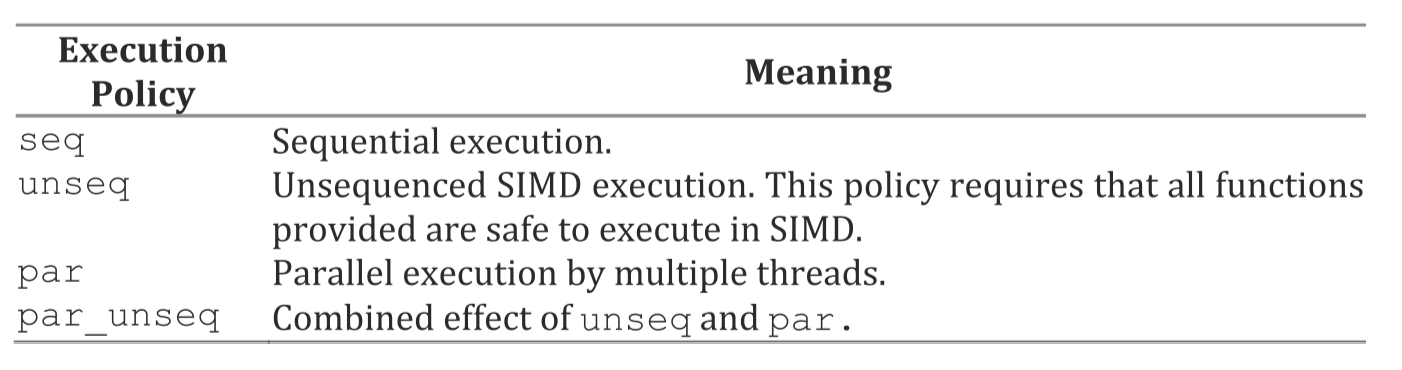
\includegraphics[width=0.9\textwidth]{figs/F18.4.png}
	\caption{\textit{执行策略 }}
\end{figure}

oneDPL 扩展了标准执行策略以提供对 SYCL 设备的支持。 
这些 SYCL 感知执行策略不仅指定算法应如何执行,还指定算法应在何处执行。 
SYCLaware 策略继承了标准 C++ 执行策略,封装了 SYCL 设备或队列,并允许我们设置可选的Kernel名称。 
SYCLaware 执行策略可与所有支持符合 C++17 标准的执行策略的标准 C++ 算法一起使用。

oneDPL 不依赖于任何单个 SYCL 编译器,它旨在支持所有 SYCL 编译器。

在我们可以使用 oneDPL 及其 SYCL 感知执行策略之前,我们需要添加一些额外的头文件。 
我们包含哪些标头取决于我们打算使用的算法,一些常见的示例包括:

• \#include <oneapi/dpl/algorithm>

• \#include <oneapi/dpl/numeric>

• \#include <oneapi/dpl/memory>

\subsubsection{SYCL执行政策}
目前,只有具有并行未排序策略 (par\_unseq) 的算法才能安全卸载到 SYCL 设备。 
这种限制源于 SYCL 中工作项提供的向前进度保证,这与其他执行策略(例如 par)的要求不兼容。

使用 SYCL 执行策略分为三个步骤:

\begin{enumerate}
	\item 将 \#include <oneapi/dpl/execution> 添加到我们的代码中。

	\item 通过提供标准策略类型、作为模板参数(可选)的唯一Kernel名称的类类型
	以及以下构造函数参数之一来创建策略对象:

		SYCL 队列 SYCL 设备 SYCL 设备选择器 具有不同Kernel名称的现有策略对象

	\item 将创建的策略对象传递给算法。
\end{enumerate}

oneapi::dpl::execution::dpcpp\_default 对象是使用默认Kernel名称和默认队列创建的预定义 device\_policy。 
这可用于创建自定义策略对象,或者在调用算法时直接传递(如果默认选择足够)。

\begin{figure}[H]
	\centering
	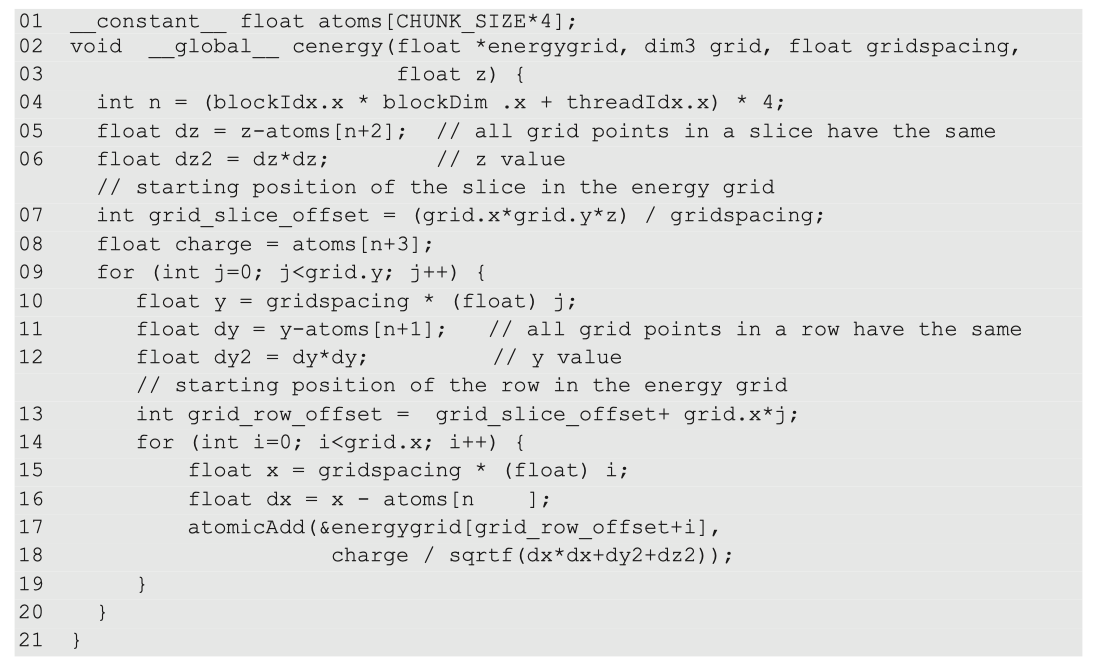
\includegraphics[width=0.9\textwidth]{figs/F18.5.png}
	\caption{\textit{创建执行策略 }}
\end{figure}

图 18-5 显示了假设使用 using 命名空间 oneapi::dpl::execution 的示例; 引用策略类和函数时的指令。

\subsubsection{将 oneDPL 与Buffer结合使用}
C++标准库中的算法都是基于迭代器的。 为了支持将 SYCL Buffer传递到这些算法中,
oneDPL 定义了两个特殊的辅助函数:oneapi::dpl::begin 和 oneapi::dpl::end。

这些函数接受 SYCL Buffer并返回满足以下要求的未指定类型的对象:

\begin{itemize}
	\item 可复制构造、可复制分配,并可与运算符 == 和 != 进行比较。

	\item 以下表达式有效:a + n、a – n 和a – b,其中a 和b 是该类型的对象,n 是整数值。

	\item 具有不带参数的get\_buffer 方法。
\end{itemize}

该方法返回传递给 oneapi::dpl::begin 和 oneapi::dpl::end 函数的 SYCL Buffer。

请注意,使用这些辅助函数需要我们将 \#include <oneapi/dpl/iterator> 添加到我们的代码中。 
默认情况下不包含此函数,因为使用 USM 时不需要这些迭代器(我们将很快重新讨论)。

\begin{figure}[H]
	\centering
	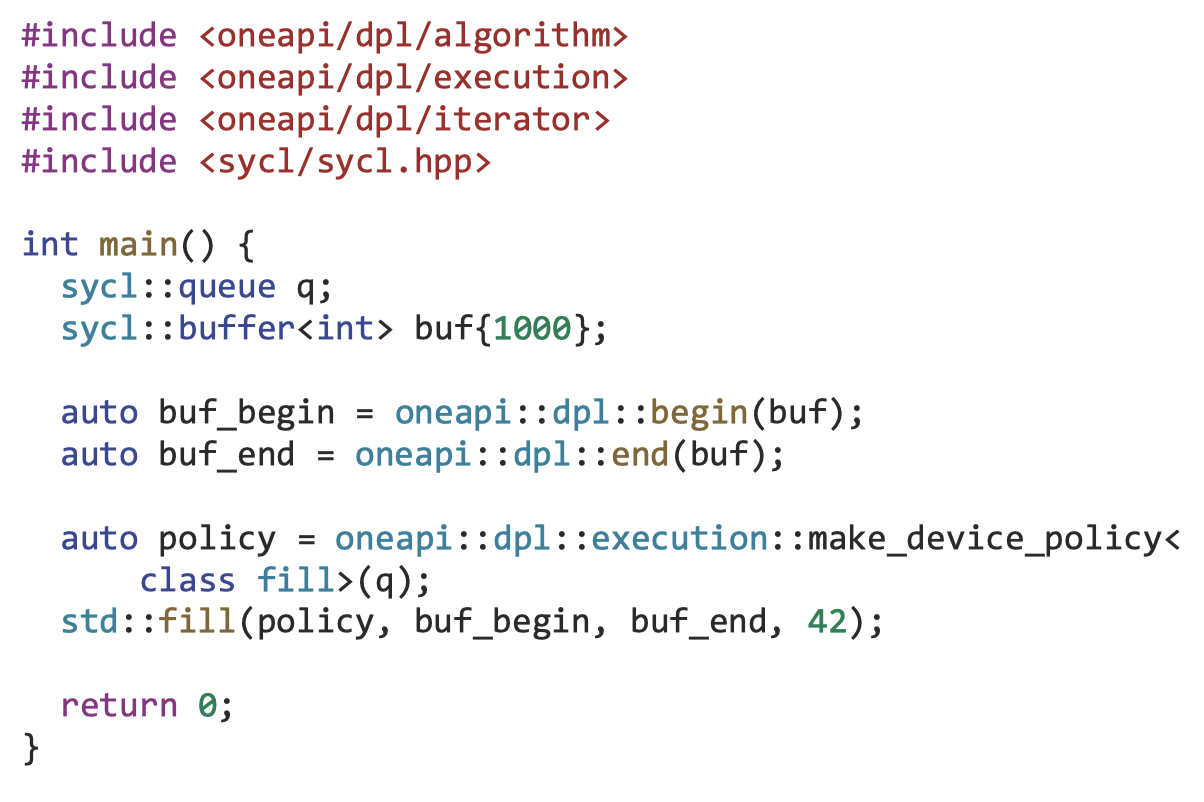
\includegraphics[width=0.9\textwidth]{figs/F18.6.png}
	\caption{\textit{使用 std::fill }}
\end{figure}

图 18-6 中的代码显示了如何将 std::fill 函数与开始/结束帮助程序结合使用来填充 SYCL Buffer。 
请注意,算法位于 std:: 命名空间中,只有执行策略位于非标准命名空间中——这不是拼写错误! 
C++ 标准库明确允许实现定义自己的执行策略来支持这样的编码模式。

\begin{figure}[H]
	\centering
	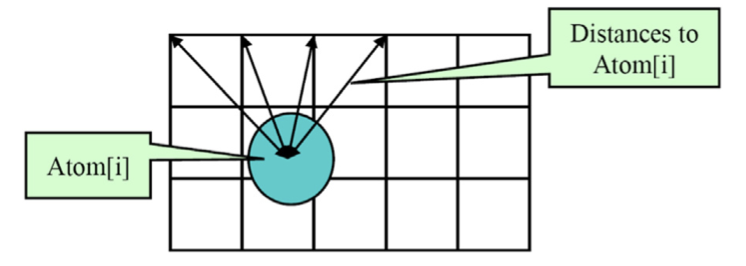
\includegraphics[width=0.9\textwidth]{figs/F18.7.png}
	\caption{\textit{将 std::fill 与默认策略和主机端迭代器结合使用 }}
\end{figure}

图 18-7 中的代码显示了该代码的更简单版本,使用默认策略和普通(主机端)迭代器。 
在这种情况下,会创建一个临时 SYCL Buffer,并将数据复制到该Buffer。 
设备上的临时Buffer处理完成后,数据将复制回主机。 
建议直接使用现有的 SYCL Buffer(如果可能),以减少主机和设备之间的数据移动以及Buffer创建和销毁的任何不必要的开销。

\begin{figure}[H]
	\centering
	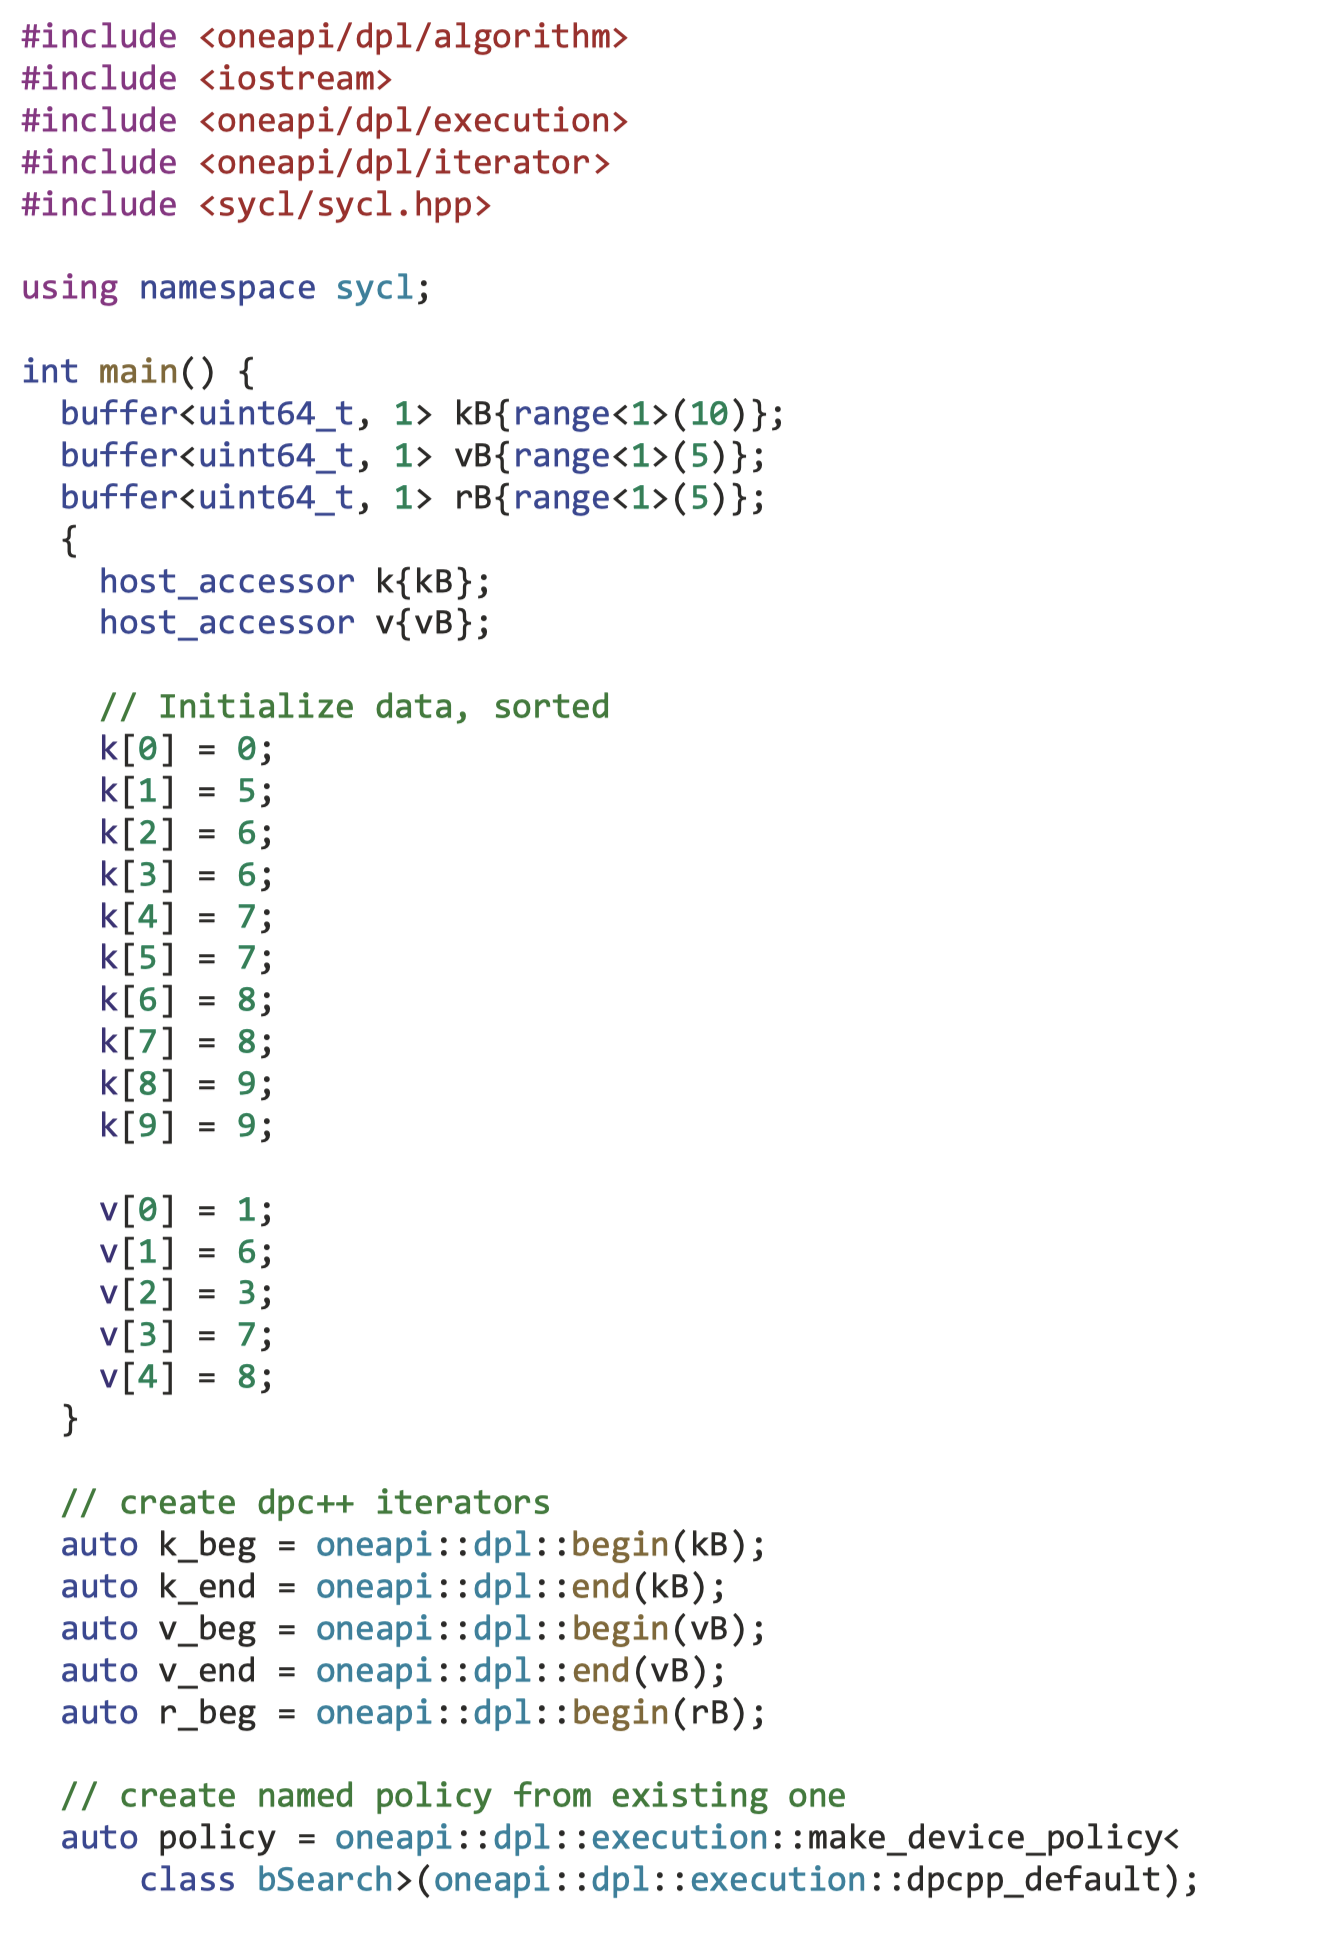
\includegraphics[width=0.9\textwidth]{figs/F18.8-1.png}
	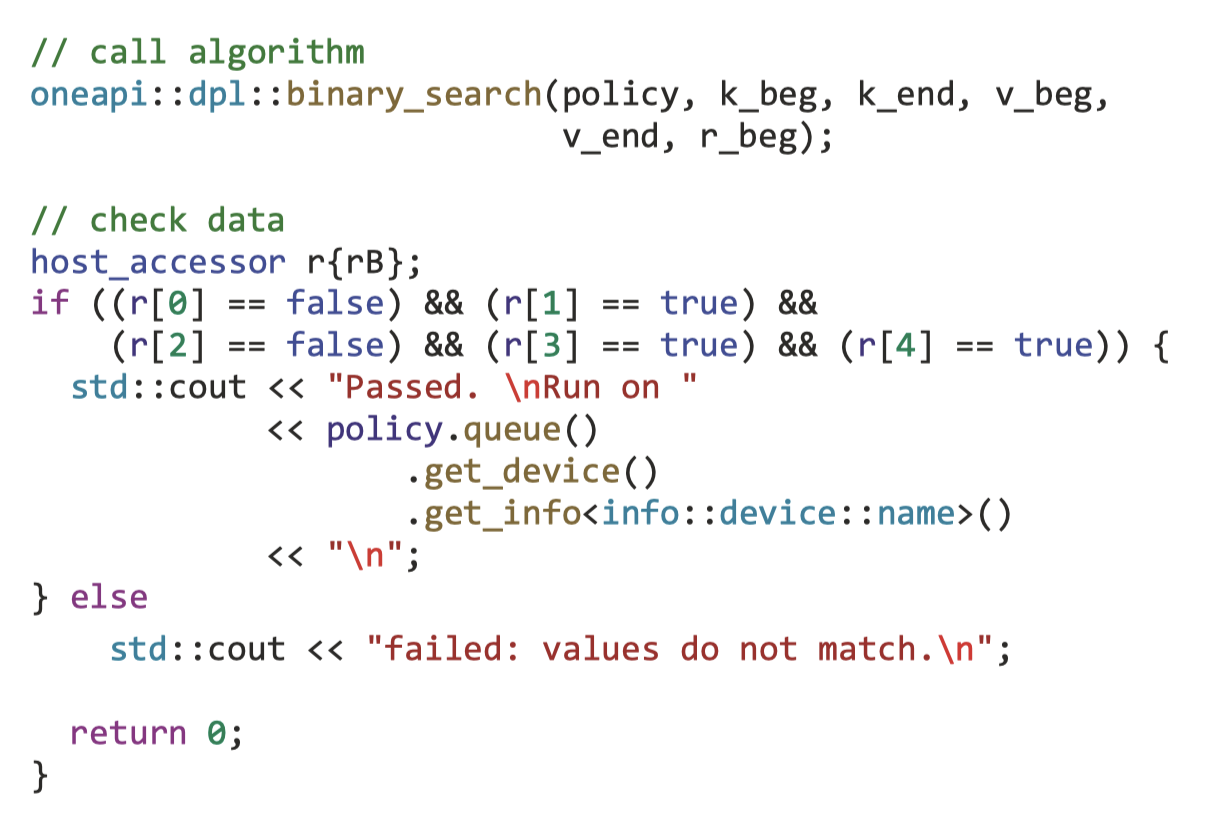
\includegraphics[width=0.9\textwidth]{figs/F18.8-2.png}
	\caption{\textit{使用 binary\_search }}
\end{figure}

图 18-8 显示了一个示例,该示例对输入序列执行二分搜索,以查找所提供的搜索序列中的每个值。 
作为搜索序列的第i个元素的搜索结果,指示是否在输入序列中找到搜索值的布尔值被分配给结果序列的第i个元素。 
该算法返回一个迭代器,该迭代器指向分配了结果的结果序列的最后一个元素。 
该算法假设输入序列已由提供的比较器排序。 如果未提供比较器,则将使用使用运算符<来比较元素的函数对象。

前面描述的复杂性强调我们应该尽可能利用库函数,而不是编写我们自己的类似算法的实现,这可能需要大量的调试和调整时间。 
我们可以利用的库的作者通常是我们所针对的设备架构内部的专家,
并且可能有权访问我们无法访问的信息,因此我们应该始终在可用时利用优化的库。

图 18-8 中所示的代码示例演示了将 oneDPL 与 SYCL Buffer结合使用时的三个典型步骤:

\begin{enumerate}
	\item 从我们的Buffer创建 SYCL 迭代器。

	\item 根据现有策略创建命名策略。

	\item 调用并行算法。
\end{enumerate}

\subsubsection{将 oneDPL 与 USM 结合使用}
在本节中,我们将探讨将 oneDPL 与 USM 结合使用的两种方法:

\begin{itemize}
	\item 通过USM 指针

	\item 通过USM 分配器
\end{itemize}

与Buffer不同,我们可以直接使用 USM 指针作为传递给算法的迭代器。 
具体来说,我们可以将指向分配开始和(过去)结束的指针传递给并行算法。 
重要的是要确保执行策略和分配本身是为同一队列或上下文创建的,以避免运行时未定义的行为。 
(请记住,这不是特定于 oneDPL 的,我们在使用 USM 时必须始终密切注意上下文!)

\begin{figure}[H]
	\centering
	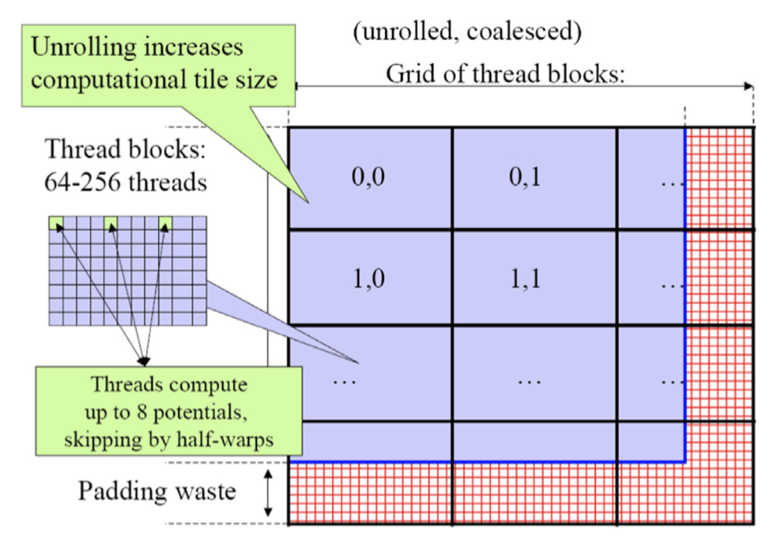
\includegraphics[width=0.9\textwidth]{figs/F18.9.png}
	\caption{\textit{将 oneDPL 与 USM 指针配合使用 }}
\end{figure}

如果相同的 USM 分配要由多个算法处理,我们可以使用有序队列或显式等待每个算法完成,
然后再在下一个算法中使用相同的分配(这是使用 USM 时的典型操作排序)。 
我们还应该小心确保在访问主机上的数据之前等待完成,如图18-9所示。

\begin{figure}[H]
	\centering
	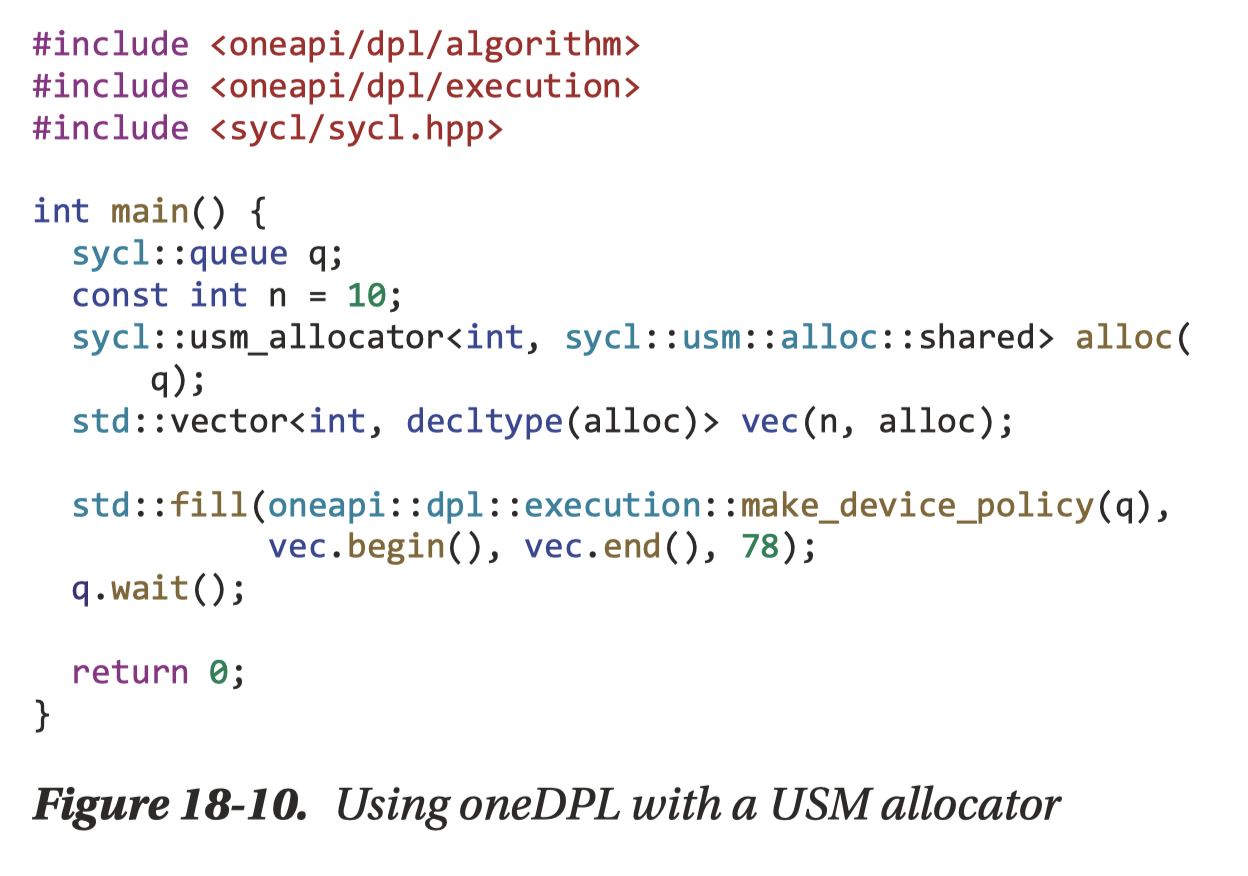
\includegraphics[width=0.9\textwidth]{figs/F18.10.png}
	\caption{\textit{将 oneDPL 与 USM 分配器配合使用 }}
\end{figure}

或者,我们可以将 std::vector 与 USM 分配器一起使用,如图 18-10 所示。 
通过这种方法,std::vector 管理自己的内存(正常情况下),
但通过对 sycl::malloc\_shared 的内部调用来分配它需要的任何内存。 
然后,begin() 和 end() 成员函数返回逐步执行 USM 分配的迭代器。 
这种编程风格非常方便,尤其是在迁移已经使用容器和算法的现有 C++ 代码时。

\subsubsection{使用 SYCL 执行策略进行错误处理}
正如第 5 章所详述的,SYCL 错误处理模型支持两种类型的错误。 
对于同步错误,运行时会引发异常,而异步错误仅在程序执行期间的指定时间由异步错误处理程序处理。

对于使用 SYCL 感知执行策略执行的算法,所有错误(同步或异步)的处理是调用者的责任。 具体来说,

\begin{itemize}
	\item 算法不会显式抛出异常。

	\item 主机CPU 上的运行时抛出的异常(包括SYCL 同步异常)将传递给调用者。

	\item SYCL 异步错误不由oneDPL 处理,因此调用者必须使用通常的SYCL 异步异常机制来处理(如果需要任何处理)。
\end{itemize}

\subsection{总结}
我们应该在异构应用程序中尽可能使用库,以避免浪费时间重写和测试通用函数和并行模式。 
我们应该利用他人的工作,而不是自己编写所有内容,
并且我们应该在可行的情况下使用这种方法来简化应用程序开发并(通常)实现卓越的性能。

本章简要介绍了我们认为每个 SYCL 开发人员都应该熟悉的三组库函数:

\begin{enumerate}
	\item SYCL内置函数,用于常见的数学运算

	\item 标准C++库,用于其他常用操作

	\item C++17并行算法(由oneDPL支持),用于完整Kernel
\end{enumerate}

对于任何库,在生产中依赖它们之前,了解哪些设备、编译器和实现经过测试和支持非常重要。 
这不是 SYCL 特定的建议,但值得记住 - 像 SYCL 这样的可移植编程解决方案的潜在目标数量巨大,
作为程序员,我们有责任确定哪些库与我们的目标一致。